% Chapter 4: Design and Implementation

\chapter{Descripción informática} % Main chapter title

\label{Chapter4} % Reference

%-------------------------------------------------------------------------------

En este capítulo se describe el desarrollo completo del proyecto, desde el diseño hasta la implementación de este, así como la metodología utilizada para la correcta evolución del mismo.

\section{Diseño}
Para la realización del desarrollo del proyecto se ha optado por seguir un paradigma de programación orientada a objetos y se ha seguido la arquitectura que se plantea en el diagrama de clases de la figura \ref{fig:diagrama-clases}, en el que se parte de un documento principal, en este caso se trata de un script ejecutable, grasp\_main.py, que contiene la información inicial y las llamadas a las clases y métodos de estas necesarios para obtener los resultados al problema.

A continuación de este parten las clases:
 \begin{itemize}
	\item \textbf{Instance}: Esta clase contendrá toda la información relacionada con una instancia o definición de grafo del problema, la cuál se compone de la clase \textbf{Node}, que contiene toda la información relativa a un nodo, así como operaciones relacionadas con el mismo.
	\item \textbf{SolutionGrasp}: Esta clase contendrá los métodos necesarios para la implementación del algoritmo \gls{GRASP} y de la búsqueda local.
	\item \textbf{GraphUtils}: Esta clase está formada por métodos estáticos en su mayoría, y contendrá todos los métodos de utilidad relacionadas con los grafos, así como la posterior exportación a fichero de los resultados obtenidos durante el proceso. También se compone de la clase \textbf{Logger}, la cuál ayuda a configurar el sistema de registros del proyecto, con el cuál poder trazar errores y ver el estado del progreso más fácilmente.
\end{itemize}

También se encuentran las clases:
 \begin{itemize}
	\item \textbf{SolutionGreedy}: Esta clase abstracta contiene lo necesario para construir una solución completa mediante un algoritmo voráz. El término completa se refiere a los atributos density, el cuál indica la densidad del grafo del que parte la solución; clique, el cuál contiene el listado de nodos que forman parte de la solución; sol\_value, el cuál indica el valor de la solución o función objetivo; cardinality, que contiene el valor del número de nodos de la solución y compute\_time, que indica el tiempo total de computo en hallar esa solución.
	\item \textbf{SolutionGreedyRatio}: Clase especializada en la obtención del mejor candidato posible por la condición de ratio.
	\item \textbf{SolutionGreedyNeighbors}: Al igual que \textbf{SolutionGreedyRatio}, esta clase se especializa en encontrar el mejor nodo candidato pero con mayor número de nodos vecinos.
\end{itemize}


\begin{figure}[H]
	\centering
	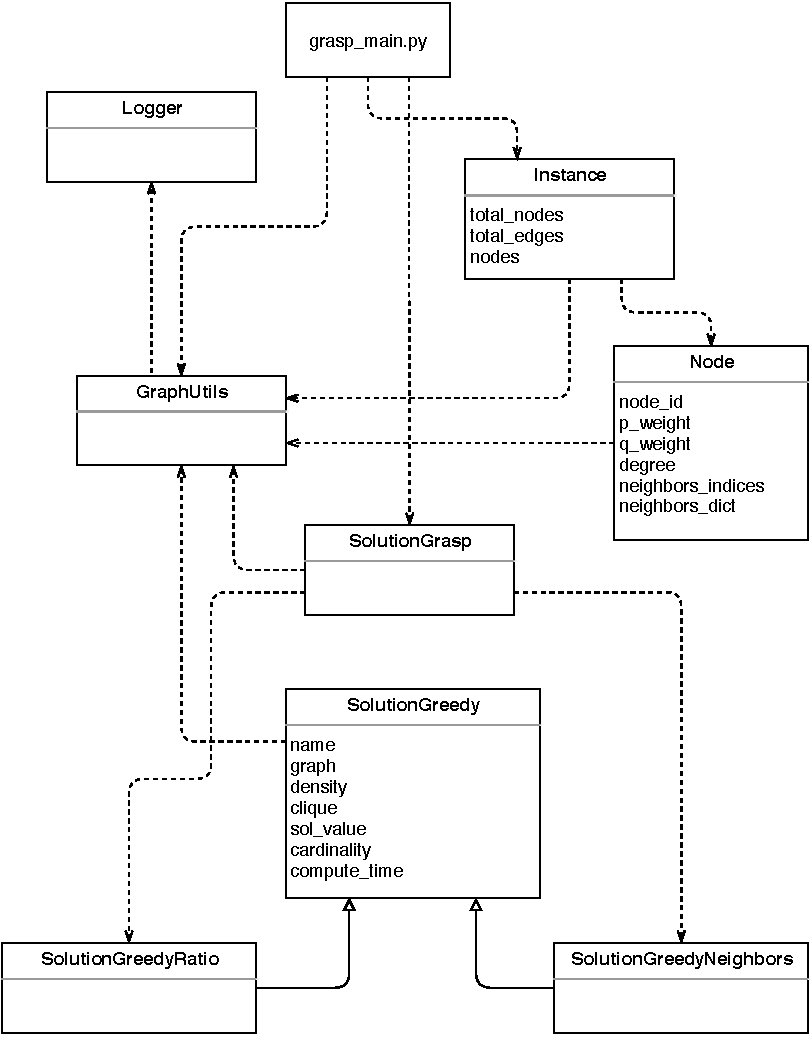
\includegraphics{Figures/Diagrama-clases.pdf}
	\caption{Diagrama de clases del proyecto.}
	\label{fig:diagrama-clases}
\end{figure}

\section{Implementación}
\label{sec:implementacion}
La implementación de este proyecto se basa en la ejecución de un script\footnote{Secuencia de ordenes o instrucciones que serán intepretadas para su ejecución.} escrito en lenguaje Python el cual parte de una clase en la que se encuentra la siguiente sentencia de código:
 \begin{lstlisting}[language=Python]
 if__name__ == "__main__"
 \end{lstlisting}
 la cual posibilita la ejecución del script mediante el comando:
  \begin{lstlisting}[language=bash]
  python grasp_main.py
 \end{lstlisting} 

 Este script, en adelante Grasp Main, tiene la configuración necesaria para ajustar los parámetros del programa:
 \begin{itemize}
 	\item Número de iteraciones a realizar por cada fichero.
 	\item Ruta donde se encuentran los ficheros de definición de los grafos a procesar o instancias.
 	\item Ruta de los ficheros de resultados generados por el programa.	
 	\item Valores de $\alpha$ para ajustar la aleatoriedad del algoritmo.
 \end{itemize}

Grasp Main se encarga de recorrer recursivamente los ficheros que se encuentran en la ruta de recursos definida, y, por cada uno de los ficheros encontrados crea un objeto de tipo Instance, añadiendo la información del grafo:
 \begin{itemize}
	\item Número de nodos.
	\item Número de aristas.
	\item Estructura de datos con los nodos del grafo.
\end{itemize}

Esta estructura de datos contiene tantos objetos de tipo Node como tengo el grafo, cada uno de ellos con la siguiente información:
 \begin{itemize}
	\item Identificador del nodo.
	\item Valor del peso p.
	\item Valor de peso q.
	\item Grado del nodo.
	\item Estructura de datos con las relaciones de este nodo con otros nodos del grafo.
\end{itemize}

Tras terminar esta operación, realiza el procesado un número N de veces, según se haya definido previamente en la configuración de la aplicación, y por cada tipo de constructivo de los que dispone la aplicación, en este caso, constructivo en base al ratio de los nodos y constructivo en base al numero de nodos adyacentes, los cuales serán explicados más adelante. A partir de este punto se llama al algoritmo \gls{GRASP}, el cual se encuentra en la clase SolutionGrasp y contiene los métodos necesarios para la obtención de una solución, partiendo de la función $find\_grasp\_solution$, la cual inicializa los siguientes datos:
\begin{itemize}
	\item vertex, el cuál es obtenido de manera aleatoria entre todos los nodos del grafo.
	\item solution, conjunto inicializado con el vértice obtenido anteriormente.
	\item cl, lista de candidatos posibles para encontrar una solución.
\end{itemize}

Para la fase constructiva del algoritmo, la implementación se apoya en la función $get\_g$ y según el tipo elegido en la configuración inicial, se creará un objeto del constructivo específico, SolutionGreedyRatio o SolutionGreedyAdjacent. Estos heredan de la clase abstracta\footnote{En programación orientada a objetos, es un tipo de clase que no puede ser instanciada, y por lo general sirve para definir otras clases de este tipo.} SolutionGreedy, la cuál tiene la información compartida por ambos tipos, y delega la implementación de la función $find\_better$ en cada una de las clases específicas, quienes mediante un algoritmo de tipo voraz buscan una solución factible en un tiempo muy reducido.
Un vez se obtienen los resultados de los candidatos, esta lista es procesada mediante la función $get\_rcl$, la cual mediante el valor de $\mu$, calculado como se mostró en el algoritmo \ref{alg:grasp} con el valor configurado $\alpha$, permite obtener la lista de candidatos restringida.
Con esta lista restringida, el siguiente paso es escoger de manera aleatoria un nodo de esta e incluirlo en el conjunto solución, eliminando los nodos de la lista de candidatos que no son adyacentes a este, ya que no formarían una solución factible.
Esta operación es realizada hasta que la lista de candidatos esté vacía.

Para mantener cierta información en un único lugar se ha implementado la clase GraphUtils, la cuál contiene información necesaria para los grafos y métodos útiles para usarse durante el procesado de los ficheros, así como su posterior exportación a ficheros de tipo CSV en este caso para mostrar los resultados obtenidos.

Para probar las diferentes funciones del proyecto se han escrito casos de prueba mediante la librería de Python unittest\footnote{https://docs.python.org/3/library/unittest.html}, para conseguir un código tolerable a posibles fallos y mantenible.

\section{Metadología empleada}
Para el desarrollo de este proyecto se ha optado por seguir una metodología de tipo iterativa e incremental, lo que permite evolucionar el proyecto progresivamente e ir adaptando los requisitos del cliente, en este caso los tutores del proyecto, en el menor tiempo posible, mejorando así la calidad del producto final con el menor esfuerzo.

Estas iteraciones e incrementos de funcionalidad se han realizado durante todo el desarrollo del proyecto, mediante reuniones, con un lapso de aproximadamente 3 a 4 semanas entre ellas, corrigiendo errores de la iteración anterior si los hubiera y aumentando la funcionalidad del producto a entregar tanto en funcionalidad como en calidad, de esta manera se consigue una evolución progresiva y segura sobre el producto y los requerimientos que el proyecto exige.

Para mantener el control y administrar lo correspondiente sobre las tareas a realizar, las que se han realizado y las realizadas del proyecto, se ha usado el administrador de proyectos Trello\footnote{https://trello.com/es}, el cuál mediante tarjetas sobre el tablero del proyecto permite conocer las tareas del proyecto, así como su estado, detalles de la misma y añadir nuevas si fuera necesario, en la figura \ref{fig:trello-tarjetas} se muestra un ejemplo de uso del sistema de tarjetas que ofrece la herramienta.

\begin{figure}[H]
	\centering
	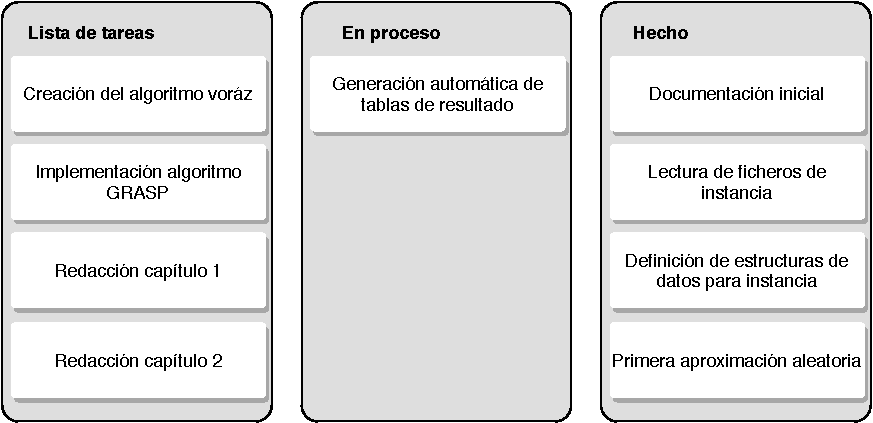
\includegraphics{Figures/trello-tarjetas.pdf}
	\caption{Ejemplo del sistema de tarjetas de Trello.}
	\label{fig:trello-tarjetas}
\end{figure}

En cuanto al mantenimiento de versiones del proyecto se ha usado el sistema de control de versiones Git\footnote{https://git-scm.com/}. Este control de versiones se ha gestionado a su vez a través del portal de alojamiento de repositorios GitHub\footnote{https://github.com/}. Para interactuar entre el repositorio local y el repositorio remoto se ha optado por hacer uso tanto de la terminal mediante los comandos del propio sistema de control de versiones Git como del cliente para tal propósito GitKraken\footnote{https://www.gitkraken.com/}, el cuál permite mediante su sencilla e intuitiva interfaz mantener un control exhaustivo sobre las ramas y versionado de las distintas piezas de código del proyecto en el que se trabaja, así como revisar posibles conflictos que se produzcan.
%-------------------------------------------------------------------------------

